% !TeX spellcheck = fr_FR
\chapter{Chapitre 4 : Résultats}

%TODO comparaisons qui soient bien justifiées et qui soient dans le même pipeline et données

%TODO Faire un chapitre sur la gestion des données et complexité de cela

\section{Prototypage}
Pour débuter le prototypage, j'ai commencé à mettre en place un réseau neuronal convolutif de régression simple qui prend en 
entrée une fenêtre de taille fixe, qui contiendra les échantillons du signal de manière séquentielle dans le temps.
Et dont le résultat est une estimation de la probabilité qu'un \gls{pe} soit présent au centre de la fenêtre analysée :

\begin{figure}[tbph!]
	\centering
	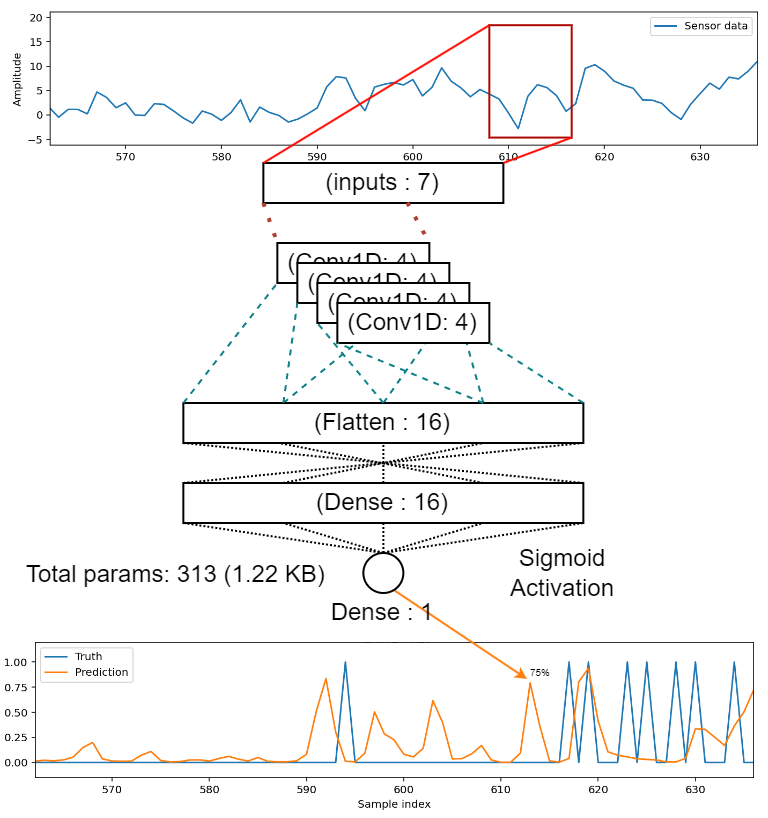
\includegraphics[width=0.6\linewidth]{cnn_simple.drawio.png}
	\caption[Diagramme de fonctionnement du premier CNN simple]{Diagramme de fonctionnement du premier CNN simple.}
\end{figure}

Le fonctionnement de cette architecture n'a pas donné de bons résultats, ceci à cause de plusieurs facteurs. Le premier est qu'à cause des paramètres
de bacs du générateur, les premiers tests effectués se basaient sur des données erronées car les impulsions n'étaient pas centrées au centre de la fenêtre.

Cette première expérience m'a aussi poussé à développer une vue au "cas par cas" où chaque inférence du modèle peut être examinée.
Cette vue affiche les données d'entrée, la vérité attendue et le résultat du modèle ce qui permet de confirmer les données d'entraînement de celui-ci. 

Cependant, même après avoir corrigé la configuration du générateur, les résultats, bien que légèrement améliorés, restaient non fiables à cause de beaucoup de
faux positif et faux négatifs.

Pour palier à cela, au lieu d'entraîner le modèle sur une seule vérité au centre de la fenêtre analysée, ce serait sur chaque 
échantillon que le réseau neuronal donnera une estimation de la présence ou non d'un \gls{pe}.

Ce nouveau modèle a immédiatement mieux performé que le précédant :

\begin{figure}[tbph!]
	\centering
	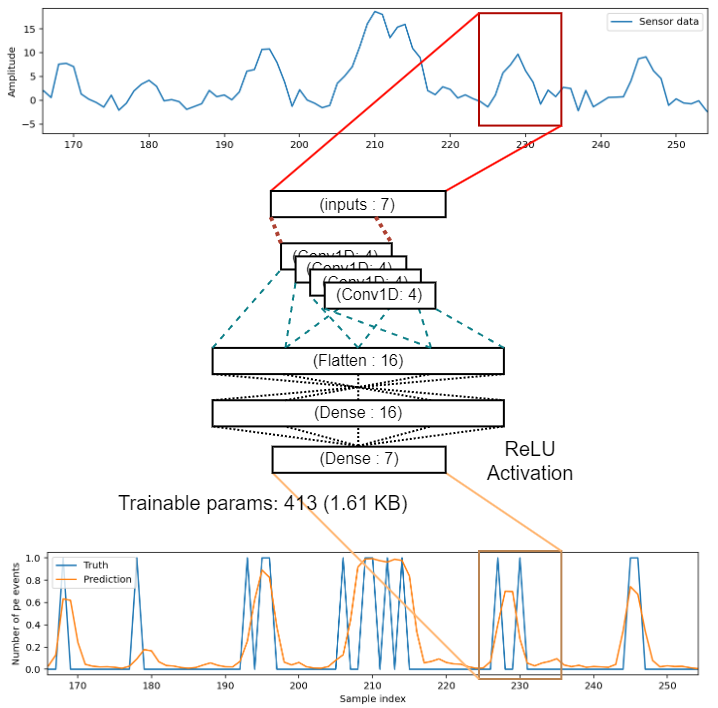
\includegraphics[width=0.6\linewidth]{cnn_mult.drawio.png}
	\caption[Diagramme de fonctionnement du deuxième CNN à multiple sortie]{Diagramme de fonctionnement du deuxième CNN à multiple sortie.}
\end{figure}

En modifiant les différents paramètres de chaque couche, il est aussi possible d'améliorer les performances de celui-ci.
De plus, en ne calculant plus la présence de manière booléenne mais en estimant la quantité de \gls{pe} présents 
en changeant la fonction d'activation finale pour utiliser la fonction mathématique "ReLU" qui n'est pas confinée 
à l'intervalle $ \left[ 0, 1\right] $ comme la sigmoïde mais à $ \left[0, +\infty\right[ $, il est possible d'entraîner le modèle
pour qu'il estime le nombre de \gls{pe} à un instant $t$ dans une fenêtre. 